\documentclass{beamer}

\usetheme{default}

\usepackage[utf8]{inputenc}
\usepackage[russian]{babel}
\usepackage{subcaption}
\captionsetup{compatibility=false}
\usepackage[many]{tcolorbox}
\usepackage{xcolor}
\renewcommand{\rmdefault}{phv}
\usepackage{listings}
\beamertemplatenavigationsymbolsempty

\makeatletter

\definecolor{otusgray}{RGB}{236, 240, 241}
\definecolor{otusdarkgray}{RGB}{53, 84, 92}
\setbeamercolor{background canvas}{bg=otusgray}
\setbeamercolor{normal text}{fg=otusdarkgray}
\setbeamercolor{title}{fg=otusdarkgray}
\setbeamertemplate{itemize items}[circle]
\setbeamercolor{itemize item}{bg=otusdarkgray,fg=otusdarkgray}
\setbeamercolor{itemize subitem}{bg=otusdarkgray,fg=otusdarkgray}



\setbeamertemplate{frametitle}
{
    \nointerlineskip
    \begin{beamercolorbox}{frametitle}
        \strut\hspace*{-0.5cm}\raisebox{-0.6cm}{
\includegraphics[width=2cm]{images/logo-small-94.png}}\strut
    \end{beamercolorbox}
}

\setbeamertemplate{footline}
{
    \nointerlineskip

    \begin{beamercolorbox}{footline}

      \begin{columns}[c]
          \begin{column}{.7\textwidth}
            \hspace*{0.3cm}
            \begin{Large} \insertframenumber \end{Large}
              \vspace{0.2cm}
          \end{column}
          \begin{column}{.3\textwidth}
            \hfill%
              \strut{
\includegraphics[width=0.9cm]{images/3434-small-242.png}}\hspace*{0.5cm}\strut
          \end{column}
      \end{columns}
    \end{beamercolorbox}
}

\newcommand{\topline}{%
  \tikz[remember picture,overlay] {%
    \draw[otusdarkgray, opacity=0.2] ([yshift=-1.1cm]current page.north west)
             -- ([yshift=-1.1cm,xshift=\paperwidth]current page.north west);
  }
}

\newcommand{\lowline}{%
  \tikz[remember picture,overlay] {%
    \draw[otusdarkgray, opacity=0.2] ([yshift=1cm]current page.south west)
             -- ([yshift=1cm,xshift=\paperwidth]current page.south west);
  }
}

\begin{document}

\defverbatim[colored]\classification{%
\begin{lstlisting}[tabsize=4,basicstyle=\ttfamily]
X, y = datasets.make_classification(
    n_features=2,
    n_informative=2,
    n_redundant=0,
    n_repeated=0,
    random_state=1
)
\end{lstlisting}
}

\defverbatim[colored]\zoloss{%
\begin{lstlisting}[tabsize=4,basicstyle=\ttfamily]
from sklearn.metrics import zero_one_loss
zero_one_loss(y, y_pred)

# 0.030000000000000027
\end{lstlisting}
}


\defverbatim[colored]\logregsklearn{%
\begin{lstlisting}[tabsize=4,basicstyle=\ttfamily]
from sklearn.linear_model import LogisticRegression
log_reg = LogisticRegression()
log_reg.fit(X, y)
y_proba = log_reg.predict_proba(X_new)
\end{lstlisting}
}

\defverbatim[colored]\logregsklearnm{%
\begin{lstlisting}[tabsize=4,basicstyle=\ttfamily]
from sklearn import linear_model, datasets
iris = datasets.load_iris()

X = iris.data[:, :2]  # we only take the first two features.
Y = iris.target
logreg = linear_model.LogisticRegression(C=1e5)
logreg.fit(X, Y)
\end{lstlisting}
}

\defverbatim[colored]\logregsklearnmresultxy{%
\begin{lstlisting}[tabsize=4,basicstyle=\ttfamily]
[[ 5.1  3.5]
 [ 4.9  3. ]
 [ 4.7  3.2]
 [ 4.6  3.1]
 [ 5.   3.6]
 [ 5.4  3.9]
 [ 4.6  3.4]
 [ 5.   3.4]
 [ 4.4  2.9]
 [ 4.9  3.1]]
[0 1 2]
\end{lstlisting}
}

\defverbatim[colored]\logregsklearnmresult{%
\begin{lstlisting}[tabsize=4,basicstyle=\ttfamily]
LogisticRegression(C=100000.0, class_weight=None,
  dual=False, fit_intercept=True,
  intercept_scaling=1, max_iter=100,
  multi_class='ovr', n_jobs=1, penalty='l2',
  random_state=None, solver='liblinear',
  tol=0.0001, verbose=0, warm_start=False)

print logreg.coef_
[[-30.619  27.55 ]
 [  0.14   -3.214]
 [  2.604  -0.743]]
\end{lstlisting}
}

\defverbatim[colored]\pseudo{%
\begin{lstlisting}[tabsize=4,basicstyle=\ttfamily]
1.function gd(X, alpha, epsilon):
2.    initialise theta
3.    do:
4.        theta = new_theta
5.        new_theta = theta - alpha * grad(X, theta)
6.    until dist(new_theta, theta) < epsilon
7.    return theta
\end{lstlisting}
}

\defverbatim[colored]\pseudost{%
\begin{lstlisting}[tabsize=4,basicstyle=\ttfamily]
1.function sgd(X, alpha, epsilon):
2. 	initialise theta
3. 	do:
4.        X = shuffle(X)
5.        for x in X:
6.            theta = new_theta
7.            new_theta = theta - alpha * grad(x, theta)
8.	until dist(new_theta, theta) < epsilon
9.	return theta
\end{lstlisting}
}

\defverbatim[colored]\sgdsklearn{%
\begin{lstlisting}[tabsize=4,basicstyle=\ttfamily]
X = iris.data[:, :2]  # we only take the first two features.
Y = iris.target
softmax_reg = LogisticRegression(multi_class="multinomial", solver="lbfgs", C=10)
softmax_reg.fit(X, Y.ravel())
\end{lstlisting}
}

\defverbatim[colored]\sgdlogregpoly{%
\begin{lstlisting}[tabsize=4,basicstyle=\ttfamily]
n_samples = 1500
x, y = datasets.make_circles(n_samples=n_samples,
    factor=.5, noise=noise)
poly_features = PolynomialFeatures(degree=2,
    include_bias=False)
X_poly = poly_features.fit_transform(x)
logit = LogisticRegression(C=c)
logit.fit(X_poly, y)
plot_boundary(...)
\end{lstlisting}
}

\defverbatim[colored]\expred{%
\begin{lstlisting}[tabsize=4,basicstyle=\ttfamily]
def predict(x, w):
    return np.sign(x.dot(w))
\end{lstlisting}
}


\defverbatim[colored]\exgd{%
\begin{lstlisting}[tabsize=4,basicstyle=\ttfamily]
for iteration in range(n_iterations):
    gradients = 2. / m * X_b.T.dot(X_b.dot(theta) - y)
    theta_old = theta
    theta = theta - alpha * gradients
    dist = np.linalg.norm(theta - theta_old)
    if dist < eps:
        break
print iteration, dist
\end{lstlisting}
}


\defverbatim[colored]\exstohgd{%
\begin{lstlisting}[tabsize=4,basicstyle=\ttfamily]
for epoch in range(n_epochs):
    p = np.random.permutation(m)
    for idx in p:
        random_index = np.random.randint(m)
        xi = X_b[[idx], :]
        yi = y[[idx], :]
        gradients = 2 * xi.T.dot(xi.dot(theta) - yi)
        theta = theta - alpha * gradients
print theta
\end{lstlisting}
}

\author{\begin{flushleft}\textbf{Ксения Стройкова} \end{flushleft}}
\date{}
\title{ \begin{flushleft}\begin{huge} \textbf{Логистическая регрессия} \end{huge} \end{flushleft}}


\begin{frame}[plain]
  
\includegraphics[width=11cm]{images/preview.jpg}
\end{frame}


\begin{frame}[plain]\frametitle{1}
  \topline
    \begin{columns}[c]
        \begin{column}{.7\textwidth}
            \maketitle
        \end{column}
        \begin{column}{.4\textwidth}
            
\includegraphics[width=4cm]{images/3434-241.png}\hspace*{-1cm}
        \end{column}
    \end{columns}
\end{frame}

\addtocounter{framenumber}{-2}

\begin{frame}\frametitle{1}
  \topline
    \begin{flushleft}\begin{Large} \textbf{Сегодня на лекции} \end{Large} \end{flushleft}

    \begin{itemize}
        \item Задачи машинного обучения, задача классификации
        \item Отступ, zero-one loss
        \item Предсказание вероятности
        \item Мультиклассовая регрессия, softmax
        \item Cross entropy
        \item Градиентный спуск
        \item Стохастический градиентный спуск
        \item Случай линейно неразделимых данных
    \end{itemize}
  \lowline
  % \footline
\end{frame}

% =======================
\section{Задачи машинного обучения, задача регрессии}
% =======================

\begin{frame}\frametitle{1}
  \topline
    \begin{flushleft}\begin{Large} \textbf{Задачи машинного обучения} \end{Large} \end{flushleft}

    \begin{itemize}
        \item Обучение с учителем
        \begin{itemize}
        \item Регрессия
        \item Классификация
        \end{itemize}
        \item Обучение без учителя
        \begin{itemize}
        \item Кластеризация
        \item Снижение размерности
        \end{itemize}
        \item Обучение с подкреплением
    \end{itemize}
  \lowline
  % \footline
\end{frame}

\begin{frame}\frametitle{1}
  \topline
    \begin{flushleft}\begin{Large} \textbf{Обучение с учителем} \end{Large} \end{flushleft}

    \begin{flushleft}есть некоторое количество примеров, для которых известны ответы\end{flushleft}

    \begin{itemize}
        \item ответы числа - регрессия
        \item ответы классы - классификация
    \end{itemize}
  \lowline
  % \footline
\end{frame}

\begin{frame}\frametitle{1}
  \topline
  \begin{flushleft}\begin{Large} \textbf{Обучение с учителем} \end{Large} \end{flushleft}
  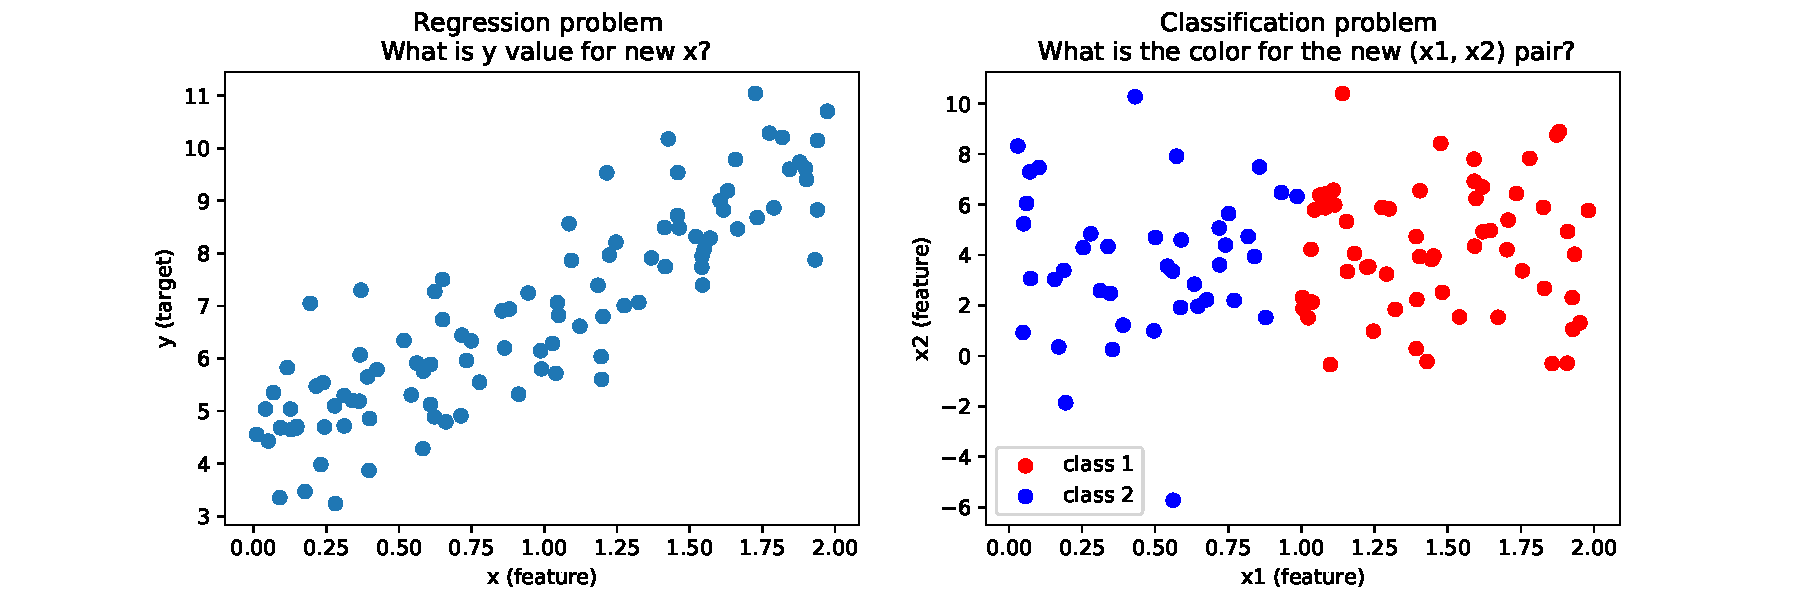
\includegraphics[width=11cm]{../pics/supervised.pdf}
  \lowline
  % \footline
\end{frame}

\begin{frame}\frametitle{1}
  \topline
    \begin{flushleft}\begin{Large} \textbf{С учителем - классификация} \end{Large} \end{flushleft}

    \classification
  \lowline
  % \footline
\end{frame}

\begin{frame}\frametitle{1}
  \topline
    \begin{flushleft}\begin{Large} \textbf{С учителем - классификация} \end{Large} \end{flushleft}

        \begin{center}
      \begin{tabular}{ l | c | r }
        \hline
       x & y  \\ \hline
       1.30022717 & -0.7856539 & 1 \\ \hline
       1.44184425 & -0.56008554 & 1\\ \hline
       -0.84792445 & -1.36621324 & 0\\ \hline
       -0.72215015 & -1.41129414 & 0\\ \hline
       -1.27221465 &  0.25945106 & 0 \\
        \hline
      \end{tabular}
    \end{center}
  \lowline
  % \footline
\end{frame}

\begin{frame}\frametitle{1}
  \topline
    \begin{flushleft}\begin{Large} \textbf{С учителем - классификация} \end{Large} \end{flushleft}

    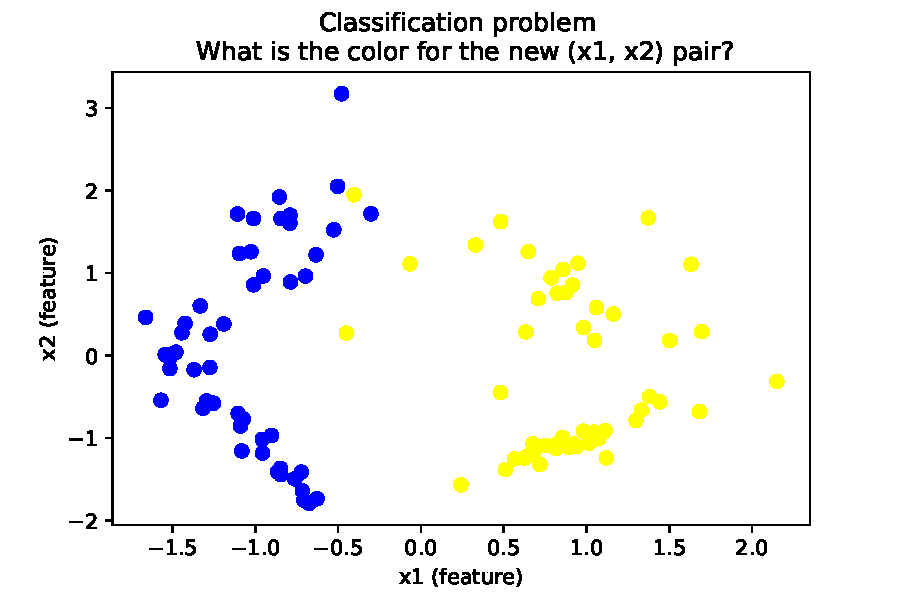
\includegraphics[width=9cm]{../pics/classification.pdf}
  \lowline
  % \footline
\end{frame}

% =======================
\section{Логистическая регрессия}
% =======================

\begin{frame}\frametitle{1}
  \topline
    \begin{flushleft}\begin{Large} \textbf{Логистическая регрессия} \end{Large} \end{flushleft}
    Построим случайную прямую.
  \lowline
  % \footline
\end{frame}

\begin{frame}\frametitle{1}
  \topline
    \begin{flushleft}\begin{Large} \textbf{Принятие решения} \end{Large} \end{flushleft}

      Простой вариант - узнать, с какой стороны от гиперплоскости находится точка
      $$\hat{y} = sign(x\theta)$$

      Уравнение прямой
      $$Ax+By+C=0$$

      Расстояние от точки $(x0, y0)$ до прямой $Ax+By+C=0$ это
      $$\frac{|Ax0 + By0 + C|}{\sqrt{(A^2 + B^2)}}$$
  \lowline
  % \footline
\end{frame}

\begin{frame}\frametitle{1}
  \topline
    \begin{flushleft}\begin{Large} \textbf{Принятие решения} \end{Large} \end{flushleft}

      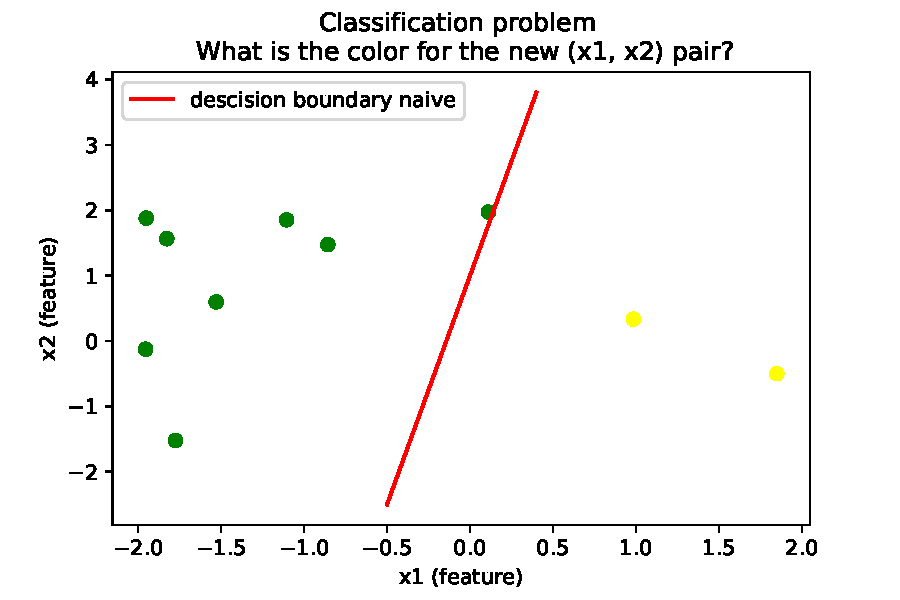
\includegraphics[width=9cm]{../pics/classification_random_line.pdf}
  \lowline
  % \footline
\end{frame}

\begin{frame}\frametitle{1}
  \topline
    \begin{flushleft}\begin{Large} \textbf{Упражнение 1} \end{Large} \end{flushleft}
      реализовать predict
  \lowline
  % \footline
\end{frame}

\begin{frame}\frametitle{1}
  \topline
    \begin{flushleft}\begin{Large} \textbf{Упражнение 1} \end{Large} \end{flushleft}
      \expred
  \lowline
  % \footline
\end{frame}

\begin{frame}\frametitle{1}
  \topline
    \begin{flushleft}\begin{Large} \textbf{Отступ - простая оценка результата} \end{Large} \end{flushleft}


      Отступ (margin) - величина $M_i = y_i \cdot x_i\theta$ (для $y = 1$ или $y = -1$), где $x_i$ - элемент обучающей выборки, $y_i$ - его класс

      $$M_i \leq 0 \Rightarrow y_i \neq \hat{y_i}$$
      $$M_i > 0 \Rightarrow y_i = \hat{y_i}$$

  \lowline
  % \footline
\end{frame}

\begin{frame}\frametitle{1}
  \topline
    \begin{flushleft}\begin{Large} \textbf{Zero-one loss} \end{Large} \end{flushleft}

Функция потерь zero-one loss:
$$ f(x) = \begin{cases}
    1, & \text{если} \space \hat{y} \neq y, \\
    0, & \text{если} \space \hat{y} = y
  \end{cases}
$$
  \lowline
  % \footline
\end{frame}

\begin{frame}\frametitle{1}
  \topline
    \begin{flushleft}\begin{Large} \textbf{Эмпирический риск - zero one loss} \end{Large} \end{flushleft}
        $$Q(\theta, x) = \frac{1}{n} \sum_{i=1}^{n} f(x) = \frac{1}{n} \sum_{i=1}^{n}[M_i < 0]$$
  \lowline
  % \footline
\end{frame}

\begin{frame}\frametitle{1}
  \topline
    \begin{flushleft}\begin{Large} \textbf{Эмпирический риск - zero one loss} \end{Large} \end{flushleft}
        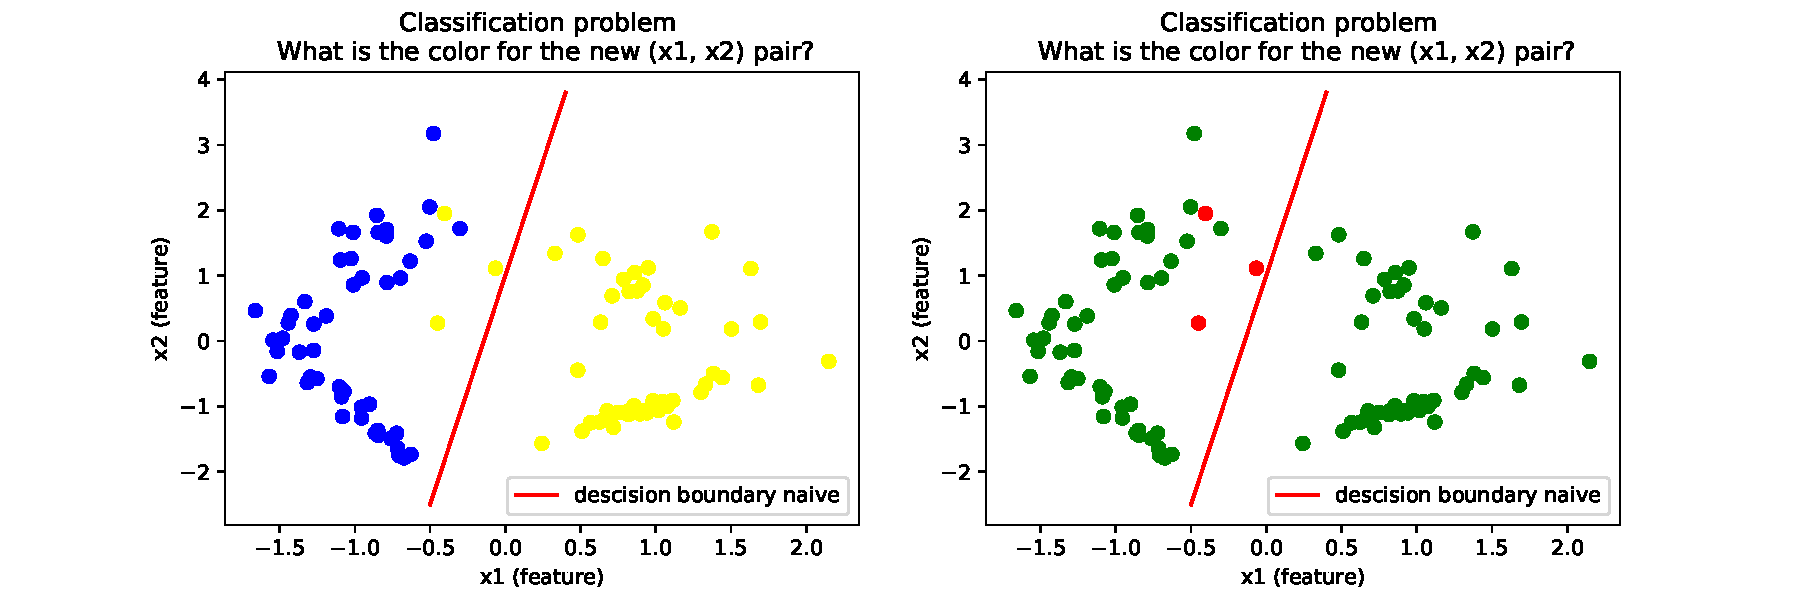
\includegraphics[width=9cm]{../pics/zero_one_loss.pdf}
  \lowline
  % \footline
\end{frame}

\begin{frame}\frametitle{1}
  \topline
    \begin{flushleft}\begin{Large} \textbf{Эмпирический риск - zero one loss} \end{Large} \end{flushleft}

      \zoloss
  \lowline
  % \footline
\end{frame}

\begin{frame}\frametitle{1}
  \topline
    \begin{flushleft}\begin{Large} \textbf{Logit regression} \end{Large} \end{flushleft}
      Переформулируем задачу
      Вместо класса будем предсказывать вероятность принадлежности классу

      $$\hat{p} = \sigma(x\theta) $$

где

$$\sigma(t)=\frac{1}{1 + exp(-t)}$$
  \lowline
  % \footline
\end{frame}

\begin{frame}\frametitle{1}
  \topline
    \begin{flushleft}\begin{Large} \textbf{Сигмоид} \end{Large} \end{flushleft}
      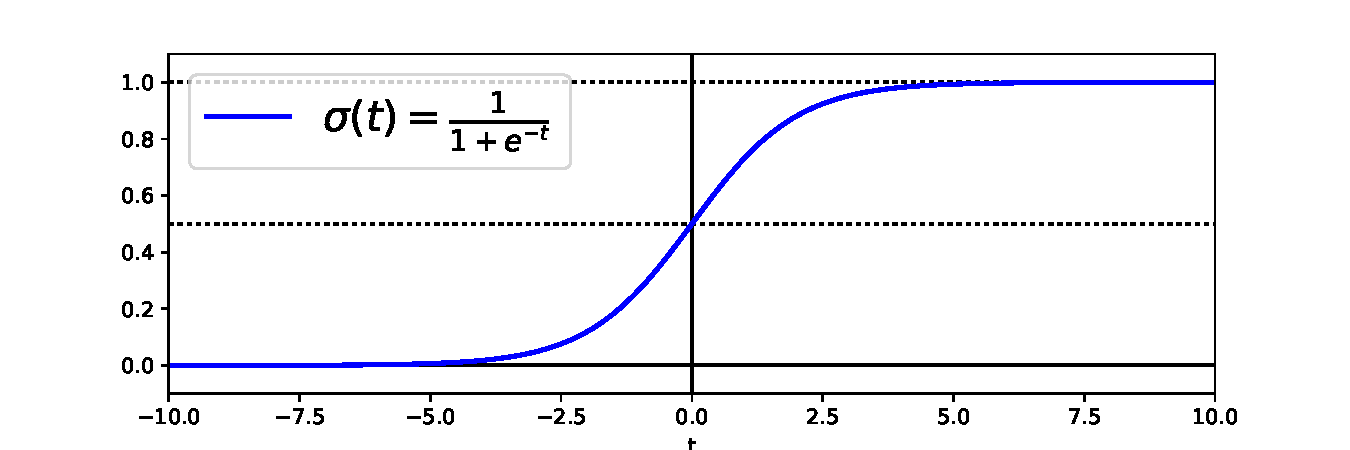
\includegraphics[width=9cm]{../pics/logistic_function_plot.pdf}
  \lowline
  % \footline
\end{frame}

\begin{frame}\frametitle{1}
  \topline
    \begin{flushleft}\begin{Large} \textbf{Предсказание} \end{Large} \end{flushleft}

$$ y = \begin{cases}
      0, & \text{если}\space \hat{p} < 0.5, \\
      1, & \text{если}\space \hat{p} \geq 0.5
    \end{cases}
$$

  \lowline
  % \footline
\end{frame}

\begin{frame}\frametitle{1}
  \topline
    \begin{flushleft}\begin{Large} \textbf{Оценка одного элемента выборки} \end{Large} \end{flushleft}

      $$ Q(\theta, x_i) = \begin{cases}
            -log(\hat{p}), & \text{если}\space y = 1, \\
            -log(1-\hat{p}), & \text{если}\space y=0
          \end{cases}
      $$

  \lowline
  % \footline
\end{frame}

\begin{frame}\frametitle{1}
  \topline
    \begin{flushleft}\begin{Large} \textbf{Для многих элементов выборки (log loss)} \end{Large} \end{flushleft}

      $$ Q(\theta, x) = - \frac{1}{m}\sum_{i=1}^{n}[y_i \log (\hat{p}_i) + (1-y_i)log(1-\hat{p}_i)]$$
  \lowline
  % \footline
\end{frame}

\begin{frame}\frametitle{1}
  \topline
    \begin{flushleft}\begin{Large} \textbf{Log loss} \end{Large} \end{flushleft}

      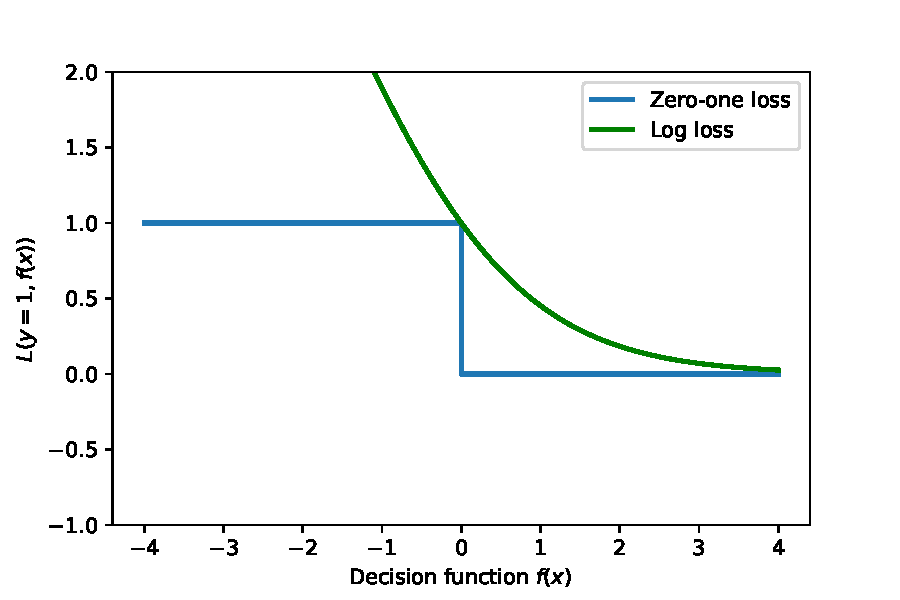
\includegraphics[width=9cm]{../pics/logloss.pdf}
  \lowline
  % \footline
\end{frame}

\begin{frame}\frametitle{1}
  \topline
    \begin{flushleft}\begin{Large} \textbf{Логистическая регрессия в sklearn} \end{Large} \end{flushleft}

      \logregsklearn
  \lowline
  % \footline
\end{frame}

\begin{frame}\frametitle{1}
  \topline
    \begin{flushleft}\begin{Large} \textbf{Логистическая регрессия в sklearn} \end{Large} \end{flushleft}

      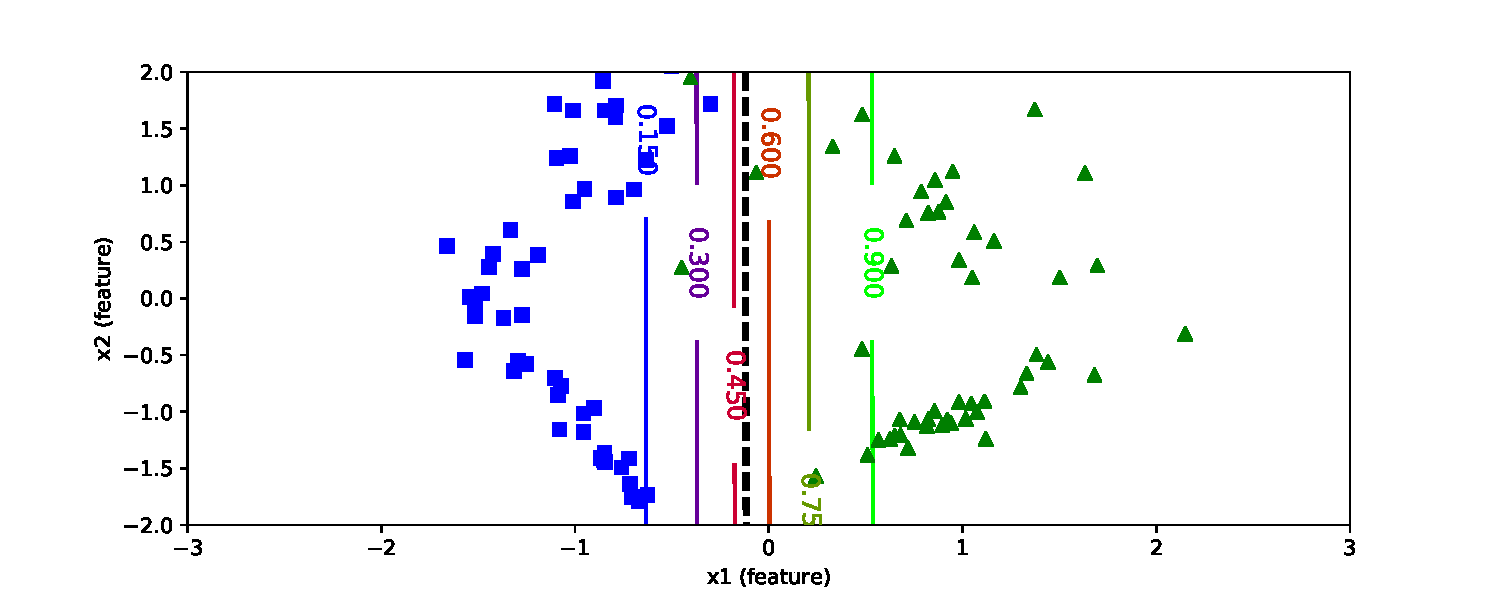
\includegraphics[width=9cm]{../pics/descision.pdf}
  \lowline
  % \footline
\end{frame}

\begin{frame}\frametitle{1}
  \topline
    \begin{flushleft}\begin{Large} \textbf{Мультиклассовая регрессия} \end{Large} \end{flushleft}

      Для обучения модели предсказывать $K$ классов можно натренировать
      \begin{itemize}
        \item $K$ классификаторов 1 против всех (one vs rest)
        \item $K(K-1)/2$ классификаторов one vs one.
      \end{itemize}
      При предсказании брать максимальное значение. Вероятности нормализуются.
  \lowline
  % \footline
\end{frame}

\begin{frame}\frametitle{1}
  \topline
    \begin{flushleft}\begin{Large} \textbf{Мультиклассовая регрессия, softmax} \end{Large} \end{flushleft}

      Нам необходимо получить значения для $k$ классов - составим матрицу параметров $\Theta$
      $$ x = \begin{bmatrix} 1 & x_{11} & ... & x_{p1} \\ 1 & x_{12} & ... & x_{p2} \\ ... & ... & ... & ... \\ 1 & x_{n1} & ... & x_{n1}
\end{bmatrix} \quad
\Theta = \begin{bmatrix} \theta_{01} &  ... & \theta_{0k} \\ \theta_{11} & ... & \theta_{1k} \\ ... & ... & ... \\ \theta_{p1} & ... & \theta_{pk} \end{bmatrix} \quad
f = \begin{bmatrix} f_{01} &  ... & f_{0k} \\ f_{11} & ... & f_{1k} \\ ... & ... & ... \\ f_{n1} & ... & f_{nk}\end{bmatrix} $$
  \lowline
  % \footline
\end{frame}

\begin{frame}\frametitle{1}
  \topline
    \begin{flushleft}\begin{Large} \textbf{Мультиклассовая регрессия, softmax} \end{Large} \end{flushleft}

      $$ \hat{p}_k = \frac{e^{x\theta_k}}{\sum_{j=1}^K e^{x\theta_j}} $$

$$ \hat{y}_k = {argmax}_k \hat{p}_k$$
  \lowline
  % \footline
\end{frame}

\begin{frame}\frametitle{1}
  \topline
    \begin{flushleft}\begin{Large} \textbf{Оценка для случая многих классов - cross entropy} \end{Large} \end{flushleft}

      $$Q(\Theta, x) = - \frac{1}{n}\sum_{i=1}^{n}\sum_{k=1}^{K} y_{ik} \log \hat{p}_{ik}$$
  \lowline
  % \footline
\end{frame}

\begin{frame}\frametitle{1}
  \topline
    \begin{flushleft}\begin{Large} \textbf{Логистическая регрессия в sklearn} \end{Large} \end{flushleft}

      \logregsklearnm
  \lowline
  % \footline
\end{frame}

\begin{frame}\frametitle{1}
  \topline
    \begin{flushleft}\begin{Large} \textbf{Логистическая регрессия в sklearn} \end{Large} \end{flushleft}

      \logregsklearnmresultxy
  \lowline
  % \footline
\end{frame}

\begin{frame}\frametitle{1}
  \topline
    \begin{flushleft}\begin{Large} \textbf{Логистическая регрессия в sklearn} \end{Large} \end{flushleft}

      \logregsklearnmresult
  \lowline
  % \footline
\end{frame}

\begin{frame}\frametitle{1}
  \topline
    \begin{flushleft}\begin{Large} \textbf{Логистическая регрессия в sklearn} \end{Large} \end{flushleft}

      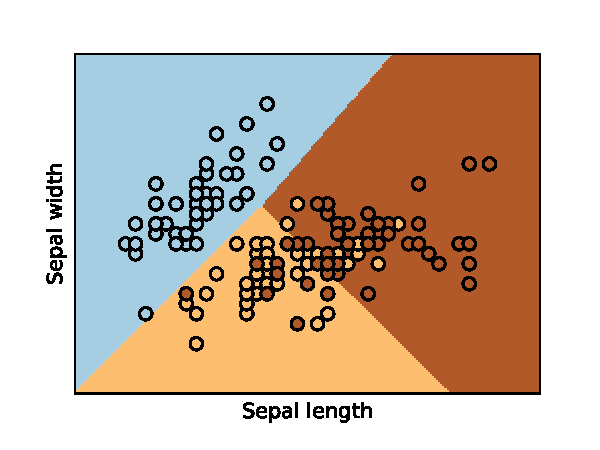
\includegraphics[width=9cm]{../pics/iris.pdf}
  \lowline
  % \footline
\end{frame}

\begin{frame}\frametitle{1}
  \topline
    \begin{flushleft}\begin{Large} \textbf{Градиентный спуск} \end{Large} \end{flushleft}

      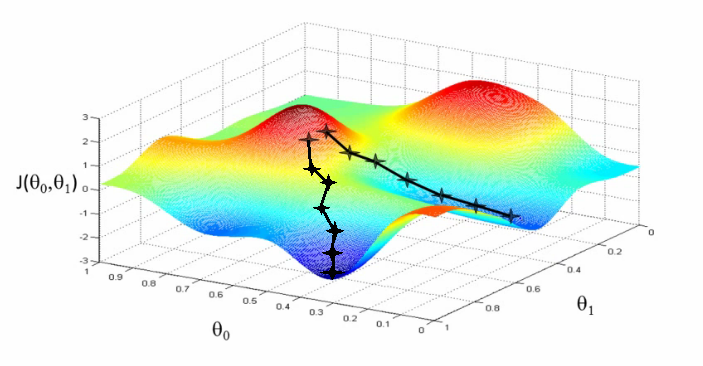
\includegraphics[width=9cm]{../pics/grad.png}
  \lowline
  % \footline
\end{frame}

\begin{frame}\frametitle{1}
  \topline
    \begin{flushleft}\begin{Large} \textbf{Градиентный спуск} \end{Large} \end{flushleft}

      $$ \theta := \theta - \alpha\frac{\partial L}{\partial \theta}$$

$\alpha$ -  скорость спуска
  \lowline
  % \footline
\end{frame}

\begin{frame}\frametitle{1}
  \topline
    \begin{flushleft}\begin{Large} \textbf{Градиент функции потерь $RSS(\theta)$} \end{Large} \end{flushleft}

      $$ RSS = \mathcal{L}(\theta) = (\hat{y} - y)^2 $$

$$ \frac{\partial L}{\partial \theta_i} = 2(\hat{y} - y)\frac{\partial L}{\partial \theta_i}(\hat{y} - y) = 2(\hat{y} - y)\frac{\partial L}{\partial \theta_i}(\theta_0x_0 + ... + \theta_1x_1 - y) = 2(\hat{y} - y)\cdot x_i$$

$$ \theta_i:= \theta_i - \alpha(\hat{y} - y)\cdot x_i$$


$\alpha$ -  скорость спуска
  \lowline
  % \footline
\end{frame}


\begin{frame}\frametitle{1}
  \topline
    \begin{flushleft}\begin{Large} \textbf{Градиент функции потерь $RSS(\theta)$} \end{Large} \end{flushleft}

      $$ \frac{\partial RSS(\theta)}{\partial \theta_i} = 2\sum_{i=1}^{n}(\theta^T\cdot x_i - y_i)x_i$$

      $$\nabla_\theta RSS(\theta) = \left( \begin{matrix} \frac{\partial L}{\partial \theta_0} \\ \frac{\partial L}{\partial \theta_1} \\ ... \\ \frac{\partial L}{\partial \theta_p} \end{matrix} \right) = x^\top(x\theta - y)$$

$\alpha$ -  скорость спуска
  \lowline
  % \footline
\end{frame}

\begin{frame}\frametitle{1}
  \topline
    \begin{flushleft}\begin{Large} \textbf{Градиент функции потерь $MSE(\theta)$} \end{Large} \end{flushleft}

$$ \frac{\partial L}{\partial \theta} = \frac{1}{n} X^\top(X\theta - y)$$
  \lowline
  % \footline
\end{frame}

\begin{frame}\frametitle{1}
  \topline
    \begin{flushleft}\begin{Large} \textbf{Псевдокод алгоритма} \end{Large} \end{flushleft}

\pseudo
  \lowline
  % \footline
\end{frame}

\begin{frame}\frametitle{1}
  \topline
    \begin{flushleft}\begin{Large} \textbf{Упражнение 2} \end{Large} \end{flushleft}

Реализовать алгоритм GD
  \lowline
  % \footline
\end{frame}


\begin{frame}\frametitle{1}
  \topline
    \begin{flushleft}\begin{Large} \textbf{Упражнение 2} \end{Large} \end{flushleft}

\exgd
  \lowline
  % \footline
\end{frame}

\begin{frame}\frametitle{1}
  \topline
    \begin{flushleft}\begin{Large} \textbf{Шаг алгоритма} \end{Large} \end{flushleft}

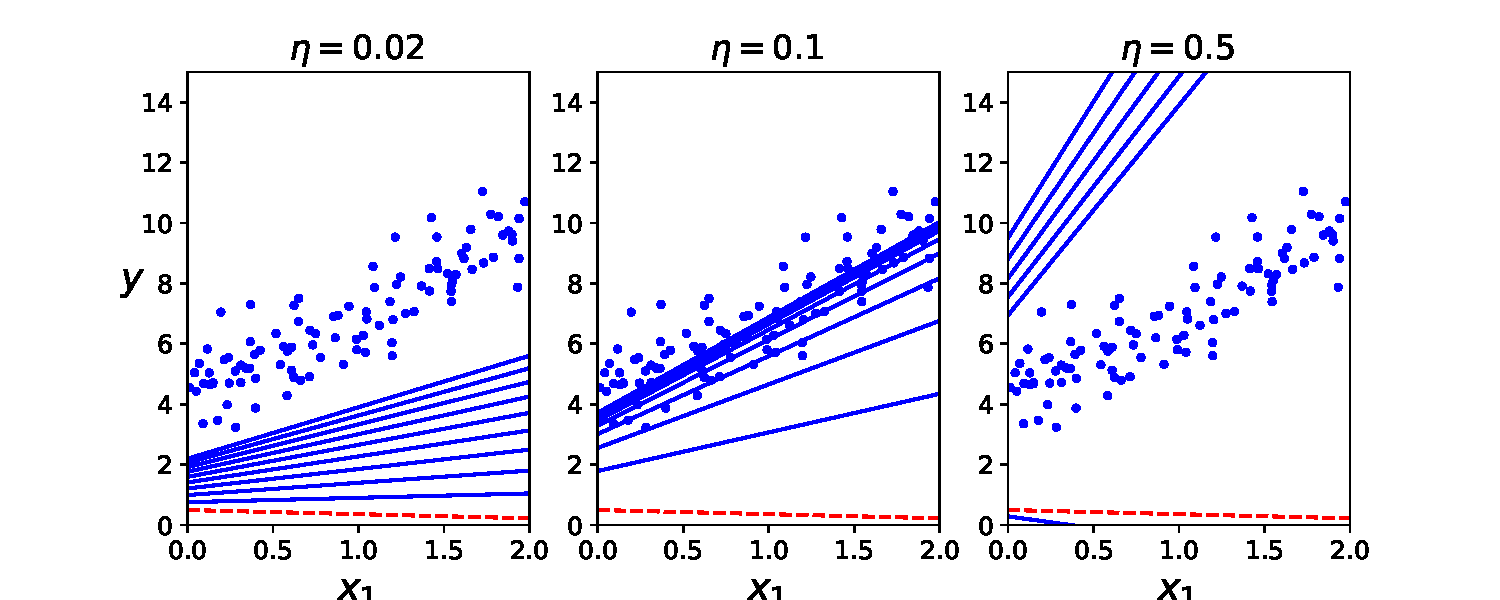
\includegraphics[width=9cm]{../pics/step.pdf}
  \lowline
  % \footline
\end{frame}

\begin{frame}\frametitle{1}
  \topline
    \begin{flushleft}\begin{Large} \textbf{Минимизация ошибки} \end{Large} \end{flushleft}

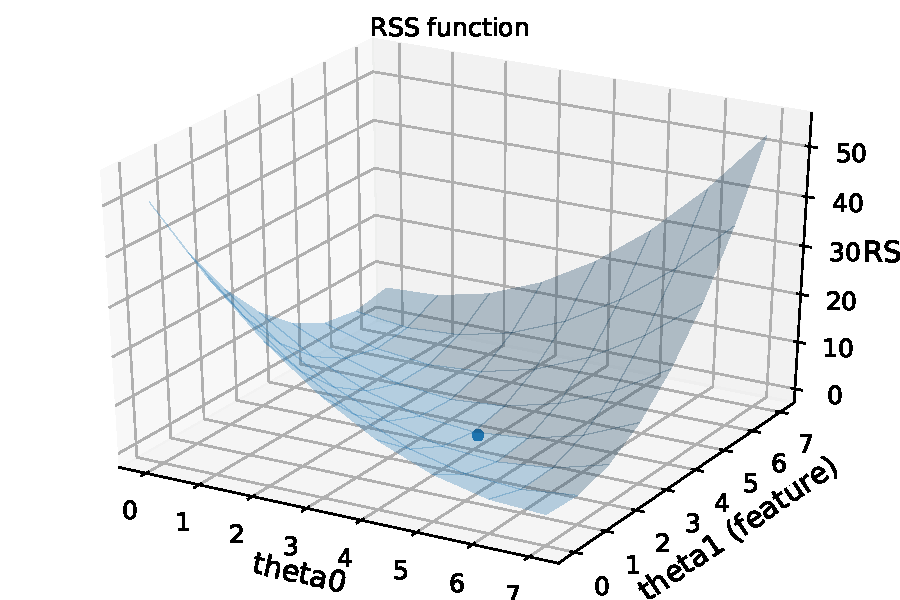
\includegraphics[width=9cm]{../pics/error_function.pdf}
  \lowline
  % \footline
\end{frame}

\begin{frame}\frametitle{1}
  \topline
    \begin{flushleft}\begin{Large} \textbf{Стохастический градиентный спуск} \end{Large} \end{flushleft}
      Проблема - используется вся обучающая выборка на каждом шаге алгоритма
Решение - использовать один случайный элемент выборки
  \lowline
  % \footline
\end{frame}

\begin{frame}\frametitle{1}
  \topline
    \begin{flushleft}\begin{Large} \textbf{Градиентный спуск} \end{Large} \end{flushleft}
      \pseudo
  \lowline
  % \footline
\end{frame}

\begin{frame}\frametitle{1}
  \topline
    \begin{flushleft}\begin{Large} \textbf{Стохастический градиентный спуск} \end{Large} \end{flushleft}
      \pseudost
  \lowline
  % \footline
\end{frame}

\begin{frame}\frametitle{1}
  \topline
    \begin{flushleft}\begin{Large} \textbf{Упражнение 3} \end{Large} \end{flushleft}
      Реализовать SGD
  \lowline
  % \footline
\end{frame}

\begin{frame}\frametitle{1}
  \topline
    \begin{flushleft}\begin{Large} \textbf{Упражнение 3} \end{Large} \end{flushleft}
      \exstohgd
  \lowline
  % \footline
\end{frame}

\begin{frame}\frametitle{1}
  \topline
    \begin{flushleft}\begin{Large} \textbf{Стохастический градиентный спуск} \end{Large} \end{flushleft}

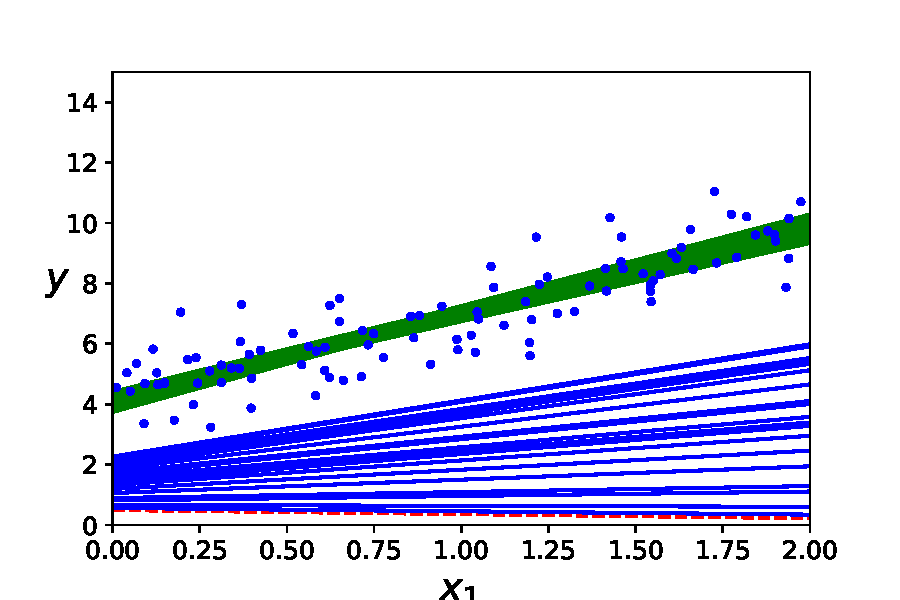
\includegraphics[width=9cm]{../pics/sgd_plot.pdf}
  \lowline
  % \footline
\end{frame}

\begin{frame}\frametitle{1}
  \topline
    \begin{flushleft}\begin{Large} \textbf{Упражнение} \end{Large} \end{flushleft}

Найти формулы для градиентного спуска для линейной регрессии с регуляризацией
  \lowline
  % \footline
\end{frame}

\begin{frame}\frametitle{1}
  \topline
    \begin{flushleft}\begin{Large} \textbf{Градиентный спуск для логистической регрессии} \end{Large} \end{flushleft}

      Бинарная классификация, log loss

      $$ Q(\theta, x) = - \frac{1}{m}\sum_{i=1}^{n}[y_i \log (\hat{p}_i) + (1-y_i)log(1-\hat{p}_i)]$$

      $$ \frac{\partial Q(\theta_j, x)}{\partial \theta_i} = \frac{1}{n} \sum_{i=1}^{n}(\sigma(\theta^T\cdot x_i) - y_i)x_ij$$
  \lowline
  % \footline
\end{frame}
\begin{frame}\frametitle{1}
  \topline
    \begin{flushleft}\begin{Large} \textbf{Градиентный спуск для логистической регрессии} \end{Large} \end{flushleft}

      cross entropy

      $$Q(\Theta, x) = - \frac{1}{n}\sum_{i=1}^{n}\sum_{k=1}^{K} y_{ik} \log \hat{p}_{ik}$$
      $$\nabla_{\theta_k}  Q(\Theta, x) = \frac{1}{n} \sum_{i=1}^{n} (\hat{p}_{ki} - y_{ki})x_i $$
  \lowline
  % \footline
\end{frame}

\begin{frame}\frametitle{1}
  \topline
    \begin{flushleft}\begin{Large} \textbf{Градиентный спуск для логистической регрессии} \end{Large} \end{flushleft}
      \sgdsklearn
  \lowline
  % \footline
\end{frame}

\begin{frame}\frametitle{1}
  \topline
    \begin{flushleft}\begin{Large} \textbf{Градиентный спуск для логистической регрессии} \end{Large} \end{flushleft}
      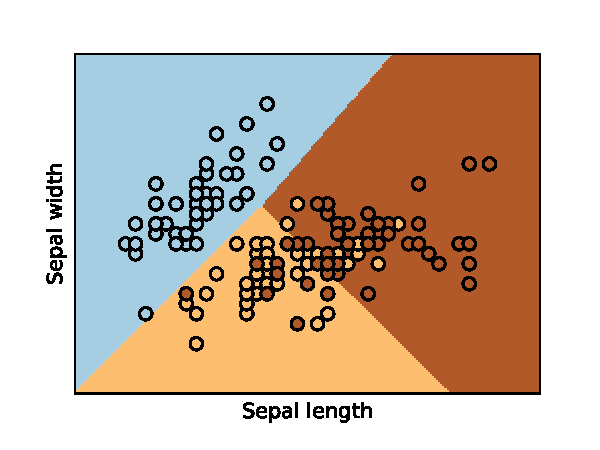
\includegraphics[width=5cm]{../pics/iris.pdf}
      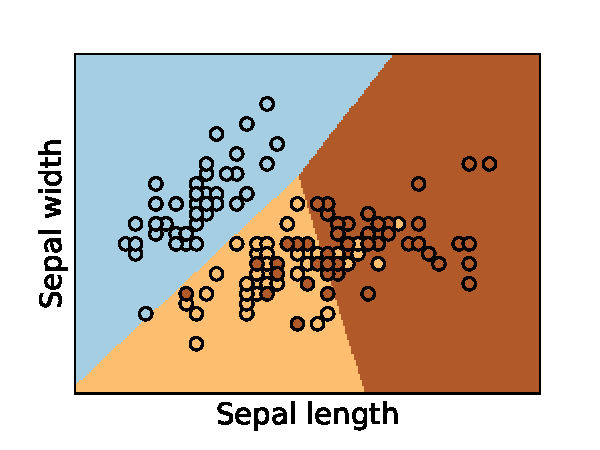
\includegraphics[width=5cm]{../pics/irissm.pdf}
  \lowline
  % \footline
\end{frame}

\begin{frame}\frametitle{1}
  \topline
    \begin{flushleft}\begin{Large} \textbf{Линейно неразделимый случай} \end{Large} \end{flushleft}
      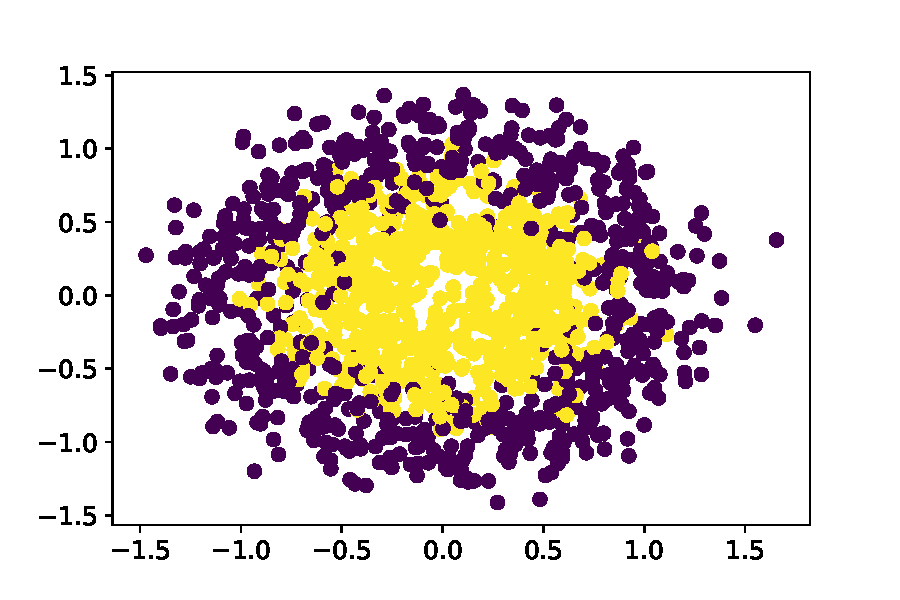
\includegraphics[width=9cm]{../pics/circles.pdf}
  \lowline
  % \footline
\end{frame}


\begin{frame}\frametitle{1}
  \topline
    \begin{flushleft}\begin{Large} \textbf{Линейно неразделимый случай} \end{Large} \end{flushleft}
      \sgdlogregpoly
  \lowline
  % \footline
\end{frame}

\begin{frame}\frametitle{1}
  \topline
    \begin{flushleft}\begin{Large} \textbf{Линейно неразделимый случай} \end{Large} \end{flushleft}
      $noise = .05$
      $c = 0.001$
      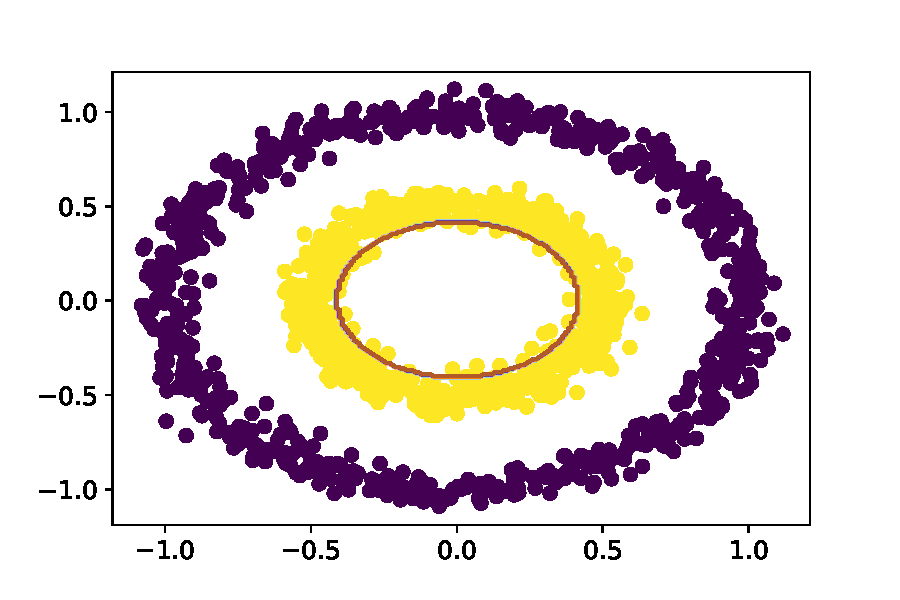
\includegraphics[width=8cm]{../pics/circles0050001.pdf}
  \lowline
  % \footline
\end{frame}

\begin{frame}\frametitle{1}
  \topline
    \begin{flushleft}\begin{Large} \textbf{Линейно неразделимый случай} \end{Large} \end{flushleft}
      $noise = .05$
      $c = 0.01$
      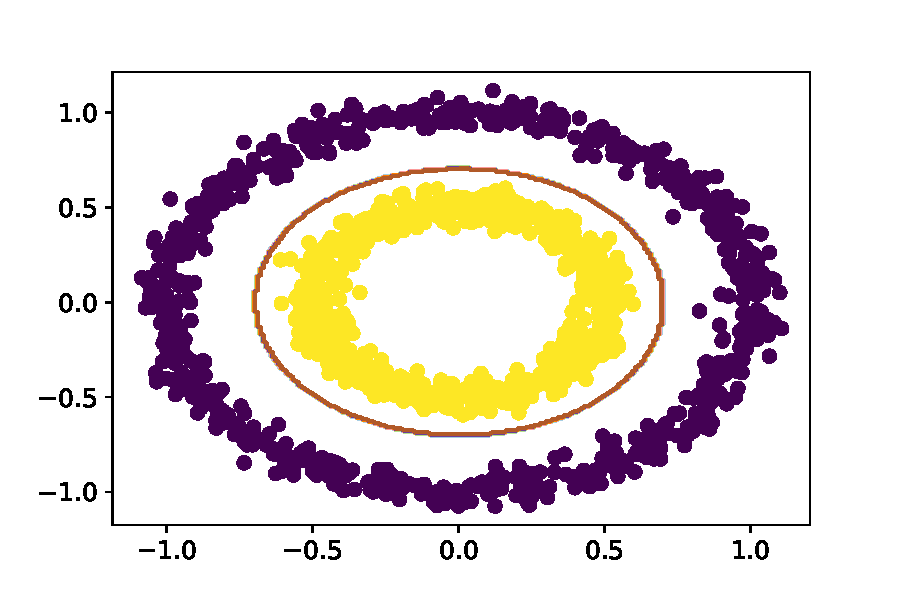
\includegraphics[width=8cm]{../pics/circles005001.pdf}
  \lowline
  % \footline
\end{frame}

\begin{frame}\frametitle{1}
  \topline
    \begin{flushleft}\begin{Large} \textbf{Линейно неразделимый случай} \end{Large} \end{flushleft}
      $noise = .05$
      $c = 0.1$
      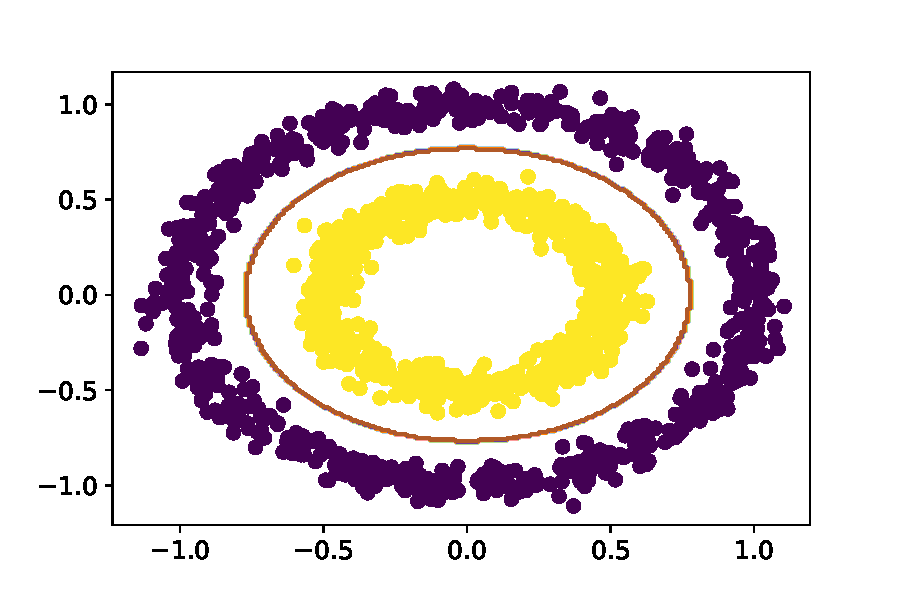
\includegraphics[width=8cm]{../pics/circles00501.pdf}
  \lowline
  % \footline
\end{frame}

\begin{frame}\frametitle{1}
  \topline
    \begin{flushleft}\begin{Large} \textbf{Линейно неразделимый случай} \end{Large} \end{flushleft}
      $noise = .05$
      $c = 1$
      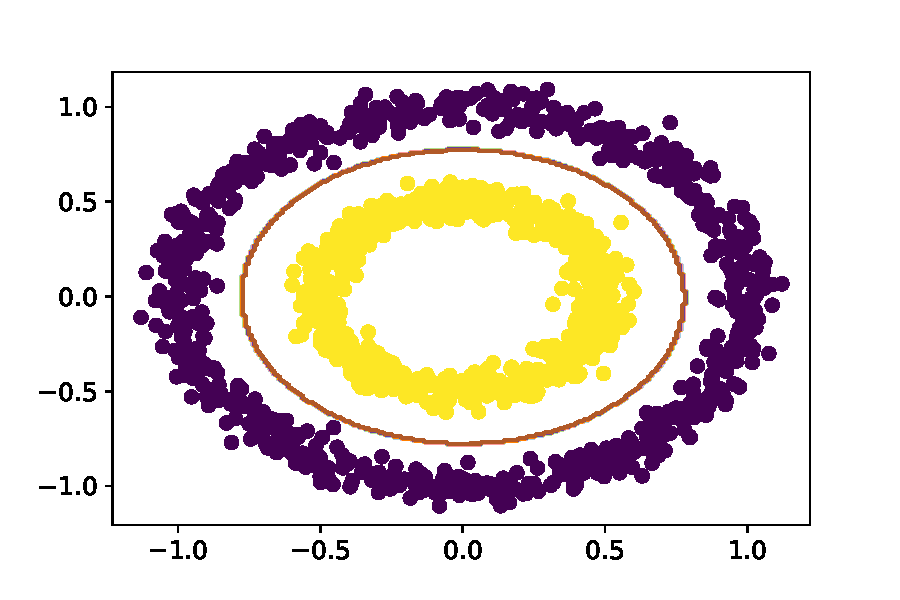
\includegraphics[width=8cm]{../pics/circles0051.pdf}
  \lowline
  % \footline
\end{frame}

\begin{frame}\frametitle{1}
  \topline
    \begin{flushleft}\begin{Large} \textbf{Линейно неразделимый случай} \end{Large} \end{flushleft}
      $noise = .20$
      $c = 0.001$
      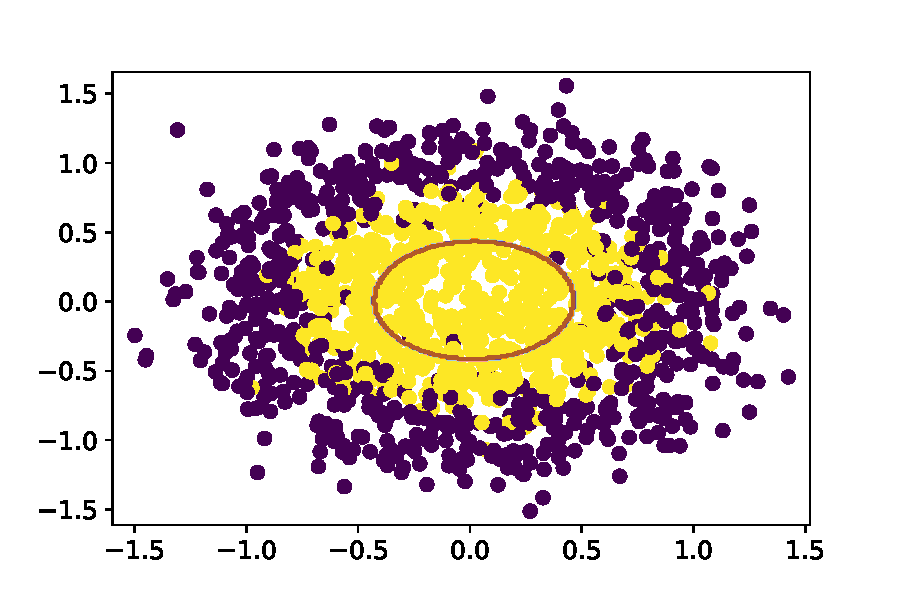
\includegraphics[width=8cm]{../pics/circles020001.pdf}
  \lowline
  % \footline
\end{frame}

\begin{frame}\frametitle{1}
  \topline
    \begin{flushleft}\begin{Large} \textbf{Линейно неразделимый случай} \end{Large} \end{flushleft}
      $noise = .20$
      $c = 0.01$
      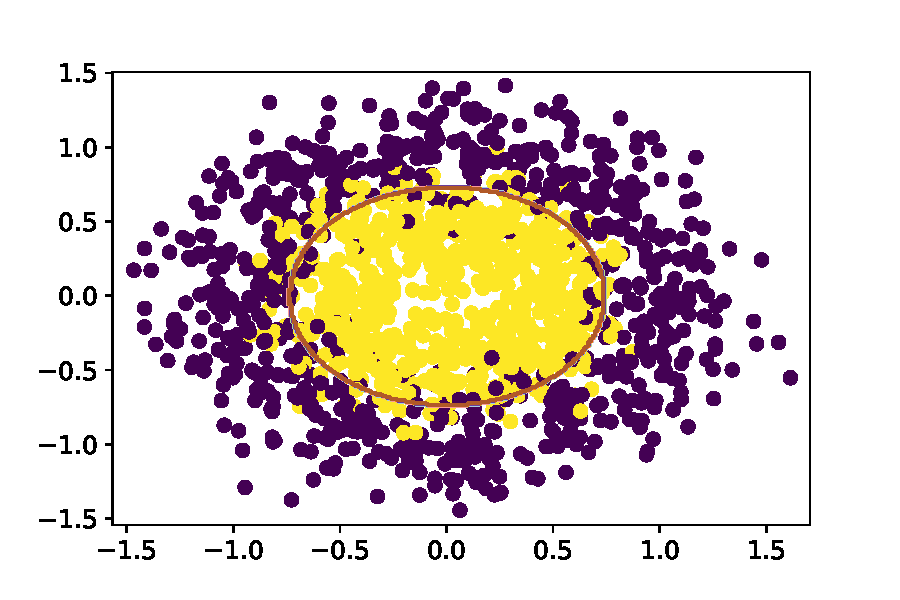
\includegraphics[width=8cm]{../pics/circles02001.pdf}
  \lowline
  % \footline
\end{frame}

\begin{frame}\frametitle{1}
  \topline
    \begin{flushleft}\begin{Large} \textbf{Линейно неразделимый случай} \end{Large} \end{flushleft}
      $noise = .20$
      $c = 0.1$
      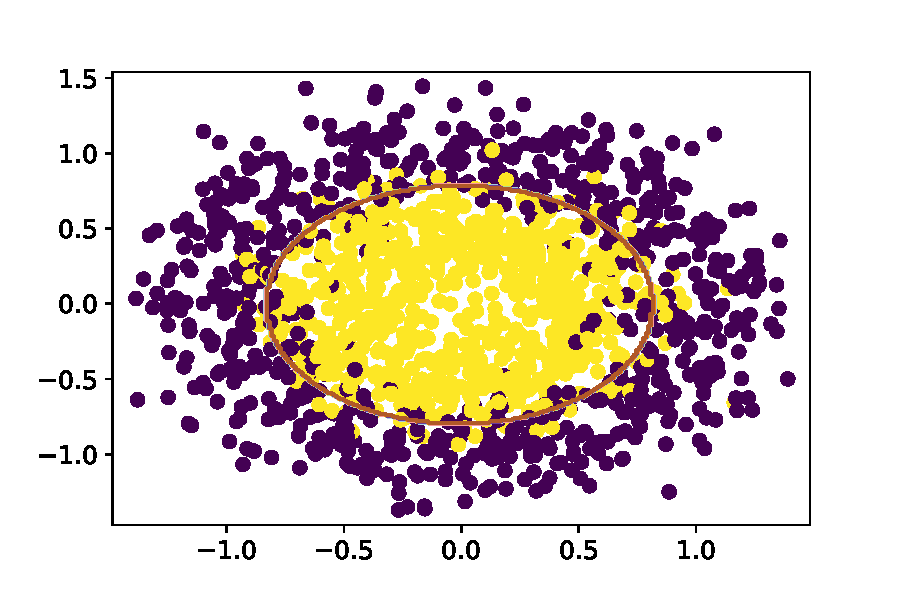
\includegraphics[width=8cm]{../pics/circles0201.pdf}
  \lowline
  % \footline
\end{frame}

\begin{frame}\frametitle{1}
  \topline
    \begin{flushleft}\begin{Large} \textbf{Линейно неразделимый случай} \end{Large} \end{flushleft}
      $noise = .20$
      $c = 1$
      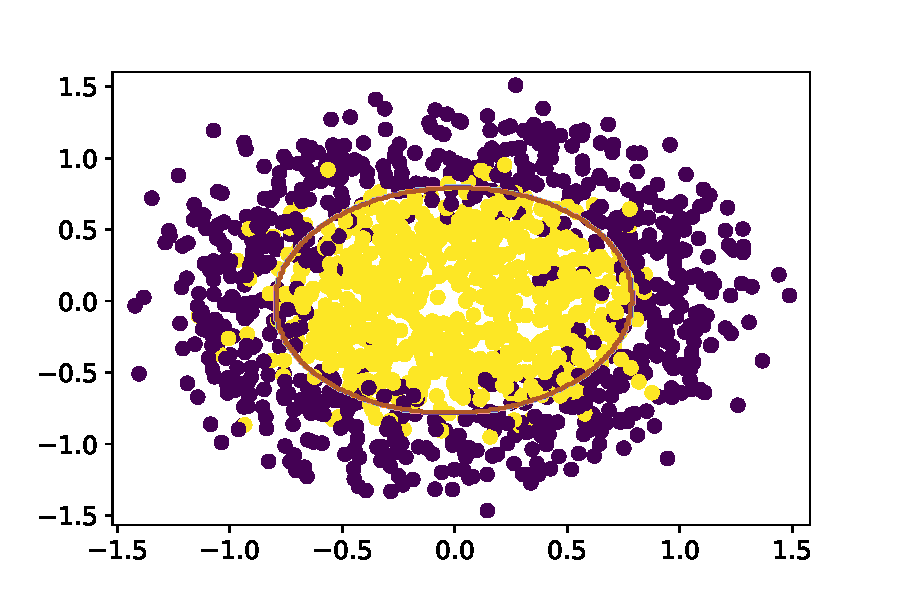
\includegraphics[width=8cm]{../pics/circles021.pdf}
  \lowline
  % \footline
\end{frame}

\begin{frame}\frametitle{1}
  \topline
    \begin{flushleft}\begin{Large} \textbf{Линейно неразделимый случай} \end{Large} \end{flushleft}
      $noise = .20$
      $c = 10000$
      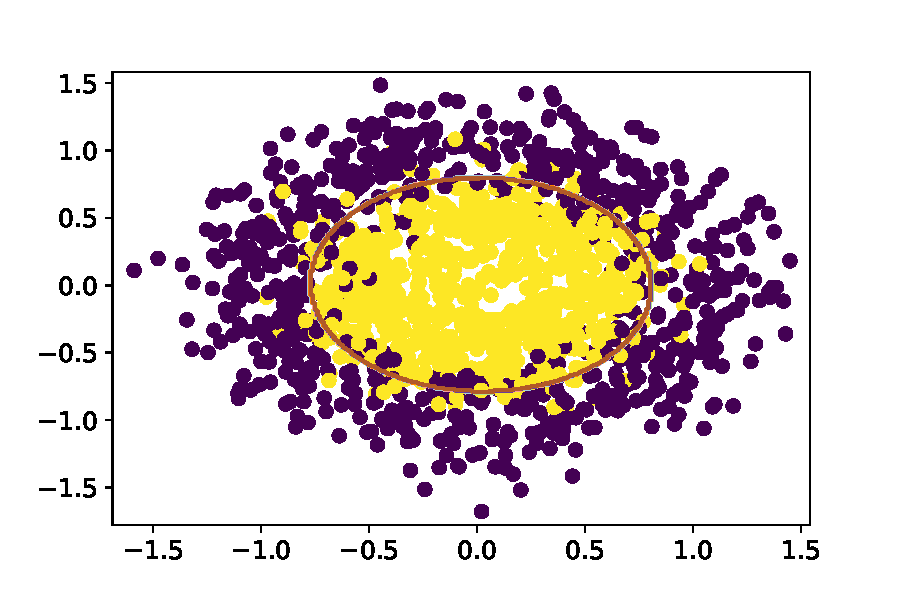
\includegraphics[width=8cm]{../pics/circles0210000.pdf}
  \lowline
  % \footline
\end{frame}

\begin{frame}\frametitle{1}
  \topline
    \begin{flushleft}\begin{Large} \textbf{Материалы} \end{Large} \end{flushleft}
        https://habrahabr.ru/company/ods/blog/322076/

Aurélien Géron - Hands-on Machine Learning with Scikit-Learn and TensorFlow
 \lowline
  % \footline
\end{frame}

\begin{frame}[plain]
\begin{center}
{\Large Вопросы}
\end{center}
\end{frame}

\end{document}
